\documentclass[conference]{IEEEtran}
\IEEEoverridecommandlockouts
% The preceding line is only needed to identify funding in the first footnote. If that is unneeded, please comment it out.
\usepackage{cite}
\usepackage{amsmath,amssymb,amsfonts}
\usepackage{algorithmic}
\usepackage{graphicx}
\usepackage{textcomp}
\usepackage{xcolor}
\usepackage{soul}

\def\BibTeX{{\rm B\kern-.05em{\sc i\kern-.025em b}\kern-.08em
    T\kern-.1667em\lower.7ex\hbox{E}\kern-.125emX}}
\begin{document}

\title{Table Tennis Analysis}

\author{\IEEEauthorblockN{1\textsuperscript{st} Pramodini Padmanaban}
\IEEEauthorblockA{\textit{Computer Science and Engineering} \\
\textit{PSG College of Technology}\\
Coimbatore, India \\
pramodheepa@gmail.com}
\and
\IEEEauthorblockN{2\textsuperscript{nd} Akash Shanmugaraj}
\IEEEauthorblockA{\textit{Computer Science and Engineering} \\
\textit{PSG College of Technology}\\
Coimbatore, India \\
akashshanmugaraj@gmail.com}
\and
\IEEEauthorblockN{3\textsuperscript{rd} Sanjitha Rajakumar}
\IEEEauthorblockA{\textit{Computer Science and Engineering} \\
\textit{PSG College of Technology}\\
Coimbatore, India \\
sanjitharajakumar@gmail.com}
\and
\IEEEauthorblockN{4\textsuperscript{th} Sreeraghavan Ramamoorthy}
\IEEEauthorblockA{\textit{Computer Science and Engineering} \\
\textit{PSG College of Technology}\\
Coimbatore, India \\
sreeraghavan16@gmail.com}
\and
\IEEEauthorblockN{5\textsuperscript{th} Dwarakesh Prasad}
\IEEEauthorblockA{\textit{Computer Science and Engineering} \\
\textit{PSG College of Technology}\\
Coimbatore, India \\
dwarakeshp@gmail.com}
}


\maketitle

\begin{abstract}
Current reasoning models heavily rely on LLMs and LLM agents taking various roles. Although this has its advantages, it requires a large number of tokens and computation. There are also other non-LLM based intelligence capabilities such as various ML models that are specialized. Using multiple specialized models in tandem is a better way to model reasoning.

This architecture facilitates flexible integration of diverse analysis components and minimizes redundant computation. A shared context layer aggregates module outputs for centralized LLM based querying and downstream applications such as visualization, summarization, and performance reporting.

We demonstrate the applicability of the system in the domain of sports video analysis, using table tennis match footage as a case study. The proposed design generalizes well to other domains that require fine-grained and interpretable video understanding.
\end{abstract}

\begin{IEEEkeywords}
component, formatting, style, styling, insert
\end{IEEEkeywords}

\section{Introduction}
Among the current mainstream approaches to reasoning, two main paradigms are tightly coupled specialized systems and generalized LLM-based systems. While tightly coupled systems perform very well in their domain, they do not expand well to other domains, and they are difficult and costly to adapt to new domains, often requiring significant re-engineering.. However, although LLMs demonstrate remarkable capabilities in diverse tasks, their reasoning is based on pattern completion rather than grounded, interpretable understanding—making them vulnerable to hallucinations or brittle reasoning.

We propose a new type of reasoning system that is decentralized in execution, scalable, and easy to modify, providing both interpretability and competitive results. By using a Publish-Subscribe model, we both reduce the amount of computation done while also implementing reasoning capabilities by having model outputs chain into messages sent to other models, mimicking AI Agent behavior in a more transparent manner.

The Mixture-of-Experts architecture is the currently used alternative. While Mixture-of-Experts architectures improve efficiency by activating only a subset of experts per input, they rely on a centralized routing mechanism and offer limited transparency into how different components contribute to the final output.

Future reasoning systems must move beyond monolithic models toward collaborative ensembles of specialized components that produce diverse inferences. These can be integrated to support richer and more context-aware insights.

This project aims to find out whether combining specialized ML models in a modular, collaborative architecture can lead to more effective and reliable intelligence than relying on an LLM alone.



\section{Problem Statement}

This project will build a scalable Table Tennis Video Analysis module—using deep‑learning models (e.g., CNNs and temporal transformers) and efficient 

spatio‑temporal feature extractors to automatically spot serve faults (net hits, illegal tosses), tally rally exchanges, pinpoint bounce locations, and produce player movement insights.

It uses the following core components - object detection, event segmentation, pose estimation, and sequence analysis. These components work together in a modular and agentic architecture, where each component functions as a semi-autonomous "agent" focused on a specialized task. Outputs from individual agents can be integrated to form higher-level insights such as:

\begin{itemize}
    \item \textbf{Player Behavioral Profiles}: Tracking trends such as preferred serve styles, stroke success rates, and movement patterns.

    \item \textbf{On-the-Fly Coaching and Feedback}: Provide point-by-point suggestions based on detected inefficiencies (e.g., slow recovery time, poor footwork on the backhand side).

    \item \textbf{Match Strategy Insights}: Recommending tactical shifts against specific opponents based on historical patterns and real-time adjustments.
\end{itemize}
The agentic architecture also allows for fast extensibility without requiring re-engineering of any core systems


\section{Literature Survey}

\subsection{Trajectory Analysis}

The research in trajectory analysis brings together a mix of classic computer vision methods and cutting-edge deep learning models. Current work explores combining videos with data from sensors like accelerometers  to create richer, more reliable information. Some ongoing challenges include dealing with missed detections when objects are hidden, reducing the effects of blurry motion, and keeping tracking smooth over time. New directions in Trajectory Analysis involve self-learning systems that don't rely on labels and neural networks inspired by physics to better predict how objects move \cite{pongball}.

\subsubsection{Workflow}

Trajectory analysis in sports follows a systematic multi-stage workflow beginning with data acquisition through high-speed cameras operating at 60-120 fps in synchronized multi-camera setups \cite{electronics14010027}. The process proceeds through intrinsic and extrinsic camera calibration using chessboard patterns and fixed reference points to establish accurate 3D coordinate systems for spatial reconstruction.

Object detection and tracking represent the core computational phase, employing models like YOLOv4, YOLOv11, and TrackNetv2 for ball detection \cite{electronics14010027}, while ByteTrack with Kalman filtering maintains temporal consistency across frames. Subsequently, 3D trajectory reconstruction utilizes triangulation for multi-camera systems or LSTM-based pipelines for monocular video \cite{pongball}, culminating in event spotting and analysis applications.

\subsubsection{Models Used}

Primary detection models include YOLOv4 and YOLOv11 for efficient small object detection, while TrackNetv2 generates heatmaps for ball localization \cite{electronics14010027}. Advanced reconstruction employs LSTM-based architectures featuring specialized networks: LSTM$\varepsilon$ for End-of-Trajectory prediction, LSTM\textsubscript{height} for vertical position estimation, and LSTM\textsubscript{refine} for trajectory smoothing.

\subsection{Stroke Analysis}

The ball is tracked in 2D---typically with YOLOv4 \cite{strokeandball}---then strokes are segmented using simple trajectory cues like local extrema and bounces. Finally, standardized trajectories feed classifiers, where Temporal Convolutional Networks excel \cite{strokeandball}, while 3D LSTM pipelines and player heatmaps add richer context beyond stroke labels.

\subsubsection{Workflow}

The workflow begins with high-quality video capture from an umpire's side view using high frame rate (around 120 fps) and 1080p resolution. Videos are processed to extract 2D ball coordinates per frame, segment continuous trajectories into strokes via mathematical rules on local extrema, and classify each stroke's type using standardized, padded, mirrored trajectory sequences \cite{strokanadball}.

Ball tracking relies primarily on a YOLOv4 detector, selected for superior F1 and fast 60 fps inference; it was pre-trained on 68,467 badminton shuttlecock images and fine-tuned on 968 table tennis ball images, leveraging the Darknet53 backbone \cite{strokaandball}. TrackNetv2, which produces heatmaps from multi-frame inputs to exploit temporal cues and handle occlusion, was also evaluated but was less preferred for this pipeline. Stroke detection uses x- and y-trajectory extrema to find temporal boundaries and ball pitches, labeling valid strokes, services, and misses.

\subsubsection{Models Used}

For recognition, deep models that preserve temporal structure performed strongest, with a Temporal Convolutional Network achieving about 87.155\% accuracy \cite{strokeandball} on pre-padded inputs and offering low variance, bias, and inference time. BiLSTM and LSTM architectures were also benchmarked.

For the classic machine learning side, each trajectory is flattened into a single feature vector. In that setup, an SVM with an RBF kernel (C=10) did best with post-padding, while KNN (k=9) was a solid pick with pre-padding. Random Forest and XGBoost were also tried \cite{strokeandball}. 3D trajectory estimates were added using an LSTM-based pipeline with three parts: predicting the end of a trajectory, estimating height, and then refining the result.

\subsection{Foul Analysis}

This work demonstrates a trajectory-centric pipeline for automated foul analysis in table tennis serves \cite{art} that couples strong detection and tracking with attention-based temporal modeling and transparent rule checks. By relying solely on 3D ball kinematics, it achieves accuracy with reduced computational cost, lowering barriers to deployment while improving referee assistance with objective, interpretable outputs grounded in physical motion cues.

\subsubsection{Workflow}

The system begins with synchronized, multi-view capture in a controlled indoor setup \cite{art} to ensure consistent lighting and reliable tracking. YOLO11 detects the fast-moving ball in each frame \cite{art}.

Triangulation fuses detections into a precise 3D trajectory with temporal indexing, which becomes the single modality driving downstream analysis. Using only trajectory and key points, the video is segmented into serve sequences and evaluated by rule-based checks on toss height, verticality, and spatial boundaries to classify frames as No Foul or Foul \cite{electronics14010027}.

\subsubsection{Models Used}

YOLO11 serves as the high-precision detector tailored for tiny, fast objects, reaching 87.52\% precision and 83.37\% recall\cite{electronics14010027} . The model's attention mechanism captures temporal structure in ballistic and post-impact motion, enabling accurate event localization without RGB or optical flow\cite{electronics14010027}. This design underpins a trajectory-only pipeline that reduces compute versus pose or multi-stream systems \cite{electronics14010027}.

\subsection{Player Heatmap}

On the player side, people were detected with Detectron2, tables found using Hough and color cues, hip positions projected into a top-down view , and movement patterns studied with heatmaps and Kolmogorov--Smirnov tests.\cite{haas2023heatmap}

\subsubsection{Workflow}

The heatmap pipeline begins with match videos of top-100 professional male players \cite{haas2023heatmap}. Active rally segments are isolated by removing replays and breaks, detecting the table via Hough transform line geometry, and filtering frames accordingly. People are detected with Detectron2; heuristics and tracking retain only the two players.

Player image-plane hip positions are projected onto the table's 3D plane to obtain a consistent top-view coordinate system centered at the table's midpoint, with continuous table tracking to handle camera motion . Aggregation and weighted normalization yield expression-specific heatmaps across attributes.\cite{haas2023heatmap}

\subsubsection{Models Used}

Table detection uses the classical Hough transform to extract straight lines \cite{haas2023heatmap}. Detectron2 performs state-of-the-art people detection; simple heuristics plus tracking isolate the two athletes. Hip keypoints are mapped from 2D images to the detected table plane, assuming hip height near table level, creating a stable top-view player position stream.

Each player's positions form an occurrence grid normalized into a probability heatmap. Analytically, heatmaps are treated as 2D probability functions and compared via a multidimensional Kolmogorov--Smirnov variant \cite{haas2023heatmap}.

\subsection{LLM Reasoning Architectures}
The blackboard model of problem solving  has historically inspired architectures that separate memory, control, and expertise\cite{hanllm}. In modern contexts, this abstraction aligns closely with large language model (LLM)-driven multi-agent systems, which integrate blackboard structures with mixture-of-experts (MoE) mechanisms\cite{hanllm}

\subsubsection{Workflow}
A typical workflow begins with a control unit—itself often an LLM—that decides which specialized agents should act based on the current problem state. These agents contribute their reasoning outputs to a shared blackboard memory, ensuring all subsequent agents operate with the same holistic context. Iterations proceed until convergence, either through consensus or predefined termination conditions.\cite{hanllm}

\subsubsection{Models Used}
Classical work by Jacobs et al. \cite{amoe} on adaptive mixtures of experts introduced the principle of dividing tasks among specialized models and dynamically weighting their outputs. This idea later scaled into architectures like the sparsely-gated MoE layer \cite{omoe}, which improved efficiency in extremely large neural networks. Recent surveys \cite{smoe} highlight how MoE structures support LLM scalability, while Han \& Zhang [14] demonstrated how coupling them with blackboard coordination improves multi-agent reasoning efficiency.

Thus, modern blackboard-based LLM multi-agent systems (bMAS) \cite{hanllm} embody a synthesis: the symbolic transparency of early blackboard systems [10], the adaptability of mixtures of experts \cite{amoe}\cite{moe}, and the scalability insights captured in surveys of MoE research \cite{moe}\cite{smoe}.

\subsection{Blackboard Architecture}

The blackboard-based LLM Multi-Agent System (bMAS) integrates the classical blackboard architecture \cite{nii1986blackboard} into LLM-driven multi-agent systems. By coordinating agents through a shared information space and adaptive scheduling, it avoids rigid workflows and inefficiencies. Its initial implementation, LbMAS, exhibits strong scalability and efficiency \cite{hanllm}.

\subsubsection{Workflow}
The blackboard-based LLM multi-agent system (bMAS) follows an iterative cycle of agent collaboration orchestrated by a control unit \cite{nii1986blackboard}. Each problem-solving session begins with agent generation, where expert roles relevant to the query are instantiated. The control unit then selects appropriate agents and supplies them with the blackboard content. Agents interpret this shared memory, contribute their outputs back to the blackboard, and the process continues until a stopping condition---consensus, a decider’s output, or maximum rounds---is achieved \cite{hanllm}.  

\subsubsection{Models Used}
The model is structured around three core components: control unit, blackboard, and LLM-based agents. The control unit, often an LLM itself, decides which agents are relevant at a given stage \cite{hanllm}, thus ensuring efficiency and reducing token consumption. The blackboard functions as shared memory, compartmentalized into public and private spaces, where agents record, debate, and refine their outputs \cite{nii1986blackboard}.  

The agents themselves perform specialized roles like problem decomposition, evaluation of inconsistencies, or solution proposal. Through repeated iterations, the system evolves towards a consensus or majority-approved solution \cite{hanllm}.

\subsection{Action Spotting}

Recent works in sports video analysis highlight how deep learning can be tailored to different game contexts. Giancola et al. (2024) addressed the challenge of action spotting in football videos by building models capable of automatically identifying temporal segments corresponding to key events, showing how large-scale video understanding can reduce reliance on manual annotations \cite{giancola}. Similarly, Voeikov et al. (2020) proposed TTNet for table tennis, a real-time framework that jointly captures temporal and spatial cues to recognize strokes and track the ball with high precision \cite{ttnet}. Together, these approaches emphasize that event localization and fine-grained spatiotemporal modeling are critical for table tennis analysis, where both rapid ball motion and subtle player actions must be detected reliably.

\section{System Design Architecture}
\begin{figure}
    \centering
    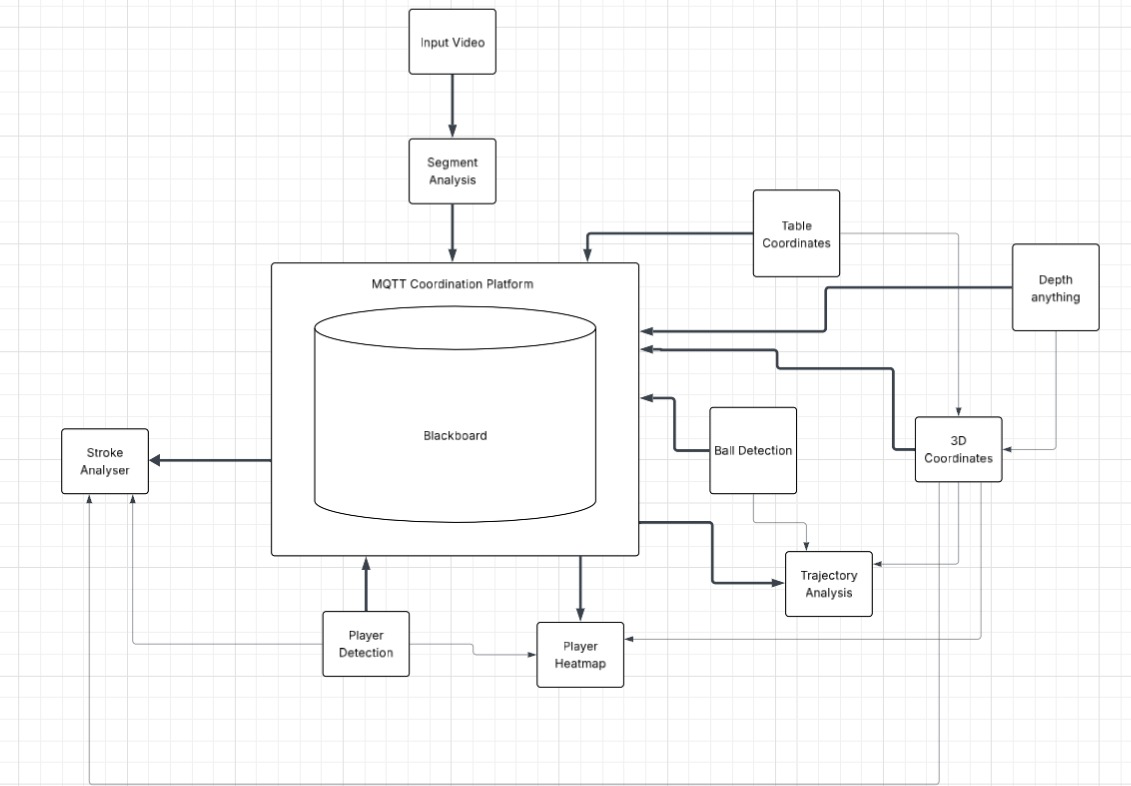
\includegraphics[width=1\linewidth]{overall-architecture.jpeg}
    \caption{Overall System Architecture Diagram}
    \label{fig:placeholder}
\end{figure}
We propose to incorporate the Blackboard Architecture (BA) into multi-agent systems (MASs) so that (1) agents with various roles can share all the information and other's messages during the whole problem-solving process, (2) agents that will take actions are selected based on the current content of the blackboard. 
This architecture allows more than just persistent memory storage and sequential function call. It enables a complex task 
solving strategy allowing different knowledge sources to communicate by the means of a common information field. 
We develop the first implementation of this proposal and conduct experiments on \hl{<>}. The results show that our system can be \hl{<>}
The overall system architecture / workflow is illustrated in Figure 1.
\subsection{Overview and Motivation}
As far back as in the 80’s of the last century, the BA was proposed \hl{(Nii, 1986; Hayes-Roth, 1985)} as a decentralized problem solving approach that imitates a group of human experts working together around a shared blackboard and each contributing her/his own solutions to the blackboard until a collective decision is reached. 
Blackboard Architecture helps a Multi-Agent System (MAS) to utilize collective intelligence to further enhance problem solving performances. 
Such a timely, iterated process enables a dynamic adaptation of collaboration mechanism among agents.
We intend to incorporate the BA into the \hl{Table Tennis} MAS and propose the blackboard-based LLM multi-agent system (bMAS) in \hl{this paper}
\subsection{Core Components}
The BA itself relies on three core components: (1) Knowledge Sources (2) Blackboard (3) Control Unit. Information from the Knowledge Sources are stored on the Blackboard and are being subsequently reused by other Knowledge Sources to iteratively approach a solution. 
\subsubsection{Blackboard}
content
\begin{figure}
    \centering
    \includegraphics[width=1\linewidth]{blackboard-class-diagram.jpeg}
    \caption{Blackboard Class Diagram}
    \label{fig:placeholder}
\end{figure}
\subsubsection{Knowledge Sources}
content
\subsubsection{Publish Subscribe Model}
content
\subsection{Component Description}
content
\subsubsection{Table Vertex Detection}
content
\subsubsection{Ball Position Detection}
content
\subsubsection{Player Heatmap Generation}
content
\subsubsection{Space Point Estimator}
content
\subsubsection{Trajectory Analysis}
content
\subsection{Interaction Model}
content
\subsection{System Workflow}
content
\section{Methodology}
content
\section{Implementation}
content
\section{Experimental Results}
\begin{table}[htbp]
\caption{Table Type Styles}
\begin{center}
\begin{tabular}{|c|c|c|c|}
\hline
\textbf{Table}&\multicolumn{3}{|c|}{\textbf{Table Column Head}} \\
\cline{2-4} 
\textbf{Head} & \textbf{\textit{Table column subhead}}& \textbf{\textit{Subhead}}& \textbf{\textit{Subhead}} \\
\hline
copy& More table copy$^{\mathrm{a}}$& &  \\
\hline
\multicolumn{4}{l}{$^{\mathrm{a}}$Sample of a Table footnote.}
\end{tabular}
\label{tab1}
\end{center}
\end{table}

% \begin{figure}[htbp]
% \centerline{\includegraphics{fig1.png}}
% \caption{Example of a figure caption.}
% \label{fig}
% \end{figure}
\section{Future Work}
The MASs proposed here so far utilizes fixed architectures with pre-defined agent roles and collaboration mechanisms, which often requires manual construction and thus lack generality.
Some recent studies develop dynamic MASs (Hu et al., 2025; Zhang et al., 2025d; Shang et al., 2025; Liu et al., 2024a; Zhang et 
al., 2025a), also called autonomous MASs, which configure structures and communication strategies based on tasks
and environment feedbacks. Such MASs are modularized and the optimized MAS configurations
are searched in specified spaces. Compared with
fixed MASs, they often have an additional, time consuming training step and the simplified search
spaces cannot cover all kinds of collaboration architectures. These two-step approaches essentially use
fixed collaboration mechanisms in problem solving
obtained from the supervised training based on a
small number of samples in the first step.
\section{Acknowledgement}
content
\bibliographystyle{plain} % or 'unsrt', 'abbrv', etc.
\bibliography{references}

\end{document}